\documentclass[10pt,a4paper]{article}
\usepackage[utf8]{inputenc}
\usepackage{amsmath}
\usepackage{amsfonts}
\usepackage{amssymb}
\usepackage{graphicx}
\usepackage{url}
\usepackage{listings}

\begin{document}

\def\File#1{\textsf{#1}}
\def\Code#1{\texttt{#1}}
\def\Key#1{\textsf{#1}}

\title{02220 Distributed systems}
\author{Kim Rostgaard Christensen (s084283)}

\maketitle

\tableofcontents

\begin{abstract}
This report describes the work done on implementing a distributed temperature monitoring network, for the course 02220 - Distributed systems using Java RMI, and apply general distributed algorithms.
\end{abstract}

\section{Introduction}
The system implemented consists of a set of inter-connected nodes that each poll a local temperature sensor at a fixed frequency. One dedicated node is appointed the role of being the master-node, or more formally the admin node. Each node (including the regular node) reports it's local sensor values back to the admin node, which then stores them.
The admin node can suffer from temporary, or permanent failures, and therefore it must be possible to promote another node to admin. This is done via a user interface which connects to the network from an external point.

\section{The system}

The overall system model of a given number of nodes. For this model we assume at least four nodes including the admin.

\subsection{Assumptions}

\begin{description}
 \item[A1] The system Contains no malicious nodes
 \item[A2] Every node has an accurate timer (not clock), so every node has the same notion of time passed, but not of absolute time
 \item[A3] A node does not change its period-count, even if disconnected.
\end{description} 

Processes cannot affect each other by other means than IPC. Processes can therefore not make other process stop/start/restart, or similar.

\subsection{Network topology}
Given the project description, a fitting topology would be the suggested fully-connected, divided into a fully connected network for doing reliable multicast, and a star-topology network for sending the temperature measurements to the admin node - which of course is the center of the star.

Upon system startup every node is given a unique identification that must be quantifiable - i.e. it must be comparable. For simplicity, a simple incrementing numbering scheme is chosen, starting from 0. The number of nodes and the topology is known before run-time by every node. This has to be done externally

\begin{figure}[h]
\centering
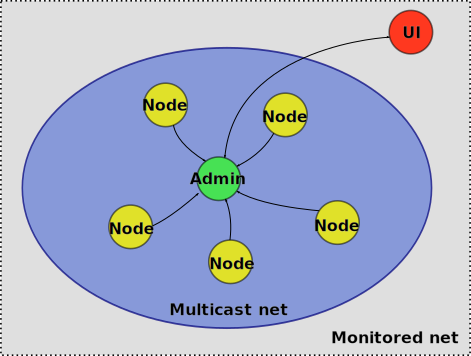
\includegraphics[scale=0.65]{fig/Networkmodel.png}
 \caption{Network model}
 \label{fig:network_model}
\end{figure}

\subsubsection{Alternate topology}
During the development of the system a number of topologies was discussed. Among these was the layered ring network, that gave some advantages when inferring causality. More details can be found in 

\subsection{Node realization}
Every node starts their life idle, and needs to be started manually using the \Code{Start()} call. For development and demonstration purposes, a bootstrapper has been developed to take care of the process launching. The bootstrapper also maintains the RMI registry, which otherwise would have to be run as separate command (\File{rmiregistry}).
Once the nodes have been started, they will register themselves as processes with their ID in the RMI registry.



\subsection{Choice of Java RMI}
As Java RMI (hereby also reference as merely RMI), doesn't really p
is used as a means to abstract away the socket-fiddling, and to ensure at-most-once semantics. In practice, the implementation introduces a single point of failure in having to have a central registry for all services. A remedial action for this could be to distribute the registry to several servers.
% Why not CORBA / RMI-IIOP?

\section{Protocol design}
%synchronization primitives with multicast.
\begin{description}
  \item[\Code{ID}:] Returns the Process ID of the remote reference as an integer.
  \item[\Code{latestAverage}:] Returns the latest average of measurements as a double-precision floating point value. This call is delegated to the current admin, if called on a regular node. The delegation is protected from infinite recursions.
  \item[\Code{sendMeasurement(TemperatureMessage)}:] Synchonously sends a temperature object embedded in a TemperatureMessage to a node. If the node is not an admin, it will reroute the message to the admin. Returns the a copy of the receivers VectorClock as a receipt.
  \item[\Code{basicDeliver(ProposedAdminMessage)}:] %TODO Returns the a copy of the receivers VectorClock as a receipt.
  \item[\Code{send(ProposedAdminMessage)}:] %TODO Returns the a copy of the receivers VectorClock as a receipt.
  \item[\Code{initialize}:] Initialize the node's internal state. Only used \emph{once} in the lifetime of a node.
  \item[\Code{startTasks}:] Start the periodic tasks of a node (see section \ref{sec:internal_tasks}). Only used \emph{once} in the lifetime of a node.
  \item[\Code{promote}:] Promotes an node to an admin (see section \ref{sec:admin_promotion}).
  \item[\Code{connectRegistry(HostString)}:] Connects the node to an RMI registry at the host supplied as argument.
  \item[\Code{disconnectRegistry}:] Disconnects a node from it's RMI registry.
\end{description} 

Each temperature object sent to the admin contains the count of the period in which it was collected.

As each admin-function related message is delegated, it removes the need for having admin-specific calls.

Furthermore there is a protocol for the network observation service, which can be seen in the file \File{ObservationServiceInterface.java}.


\subsection{Vector clocks}
Every node maintains a local vector clock that increments whenever the node changes state. This means whenever a new measurement is added, or whenever the node sends a message, the state is incremented. Whenever a node sends a message, it piggybacks its own vector clock along with the message for the receiver to merge. The receiver, upon reception of a message, sends back a receipt message containing its vector clock for the caller to merge.

- No optimizations have been done to reduce the size of vector clock messages.

\section{Admin node}
\subsection{Average temperature}
The average temperature for the user interface is an average, calculated on the basis of the latest measurements the admin has received from all nodes. To provide a consistent snapshot of the average, we have relied on \textbf{A2} and \textbf{A3}. This enables us to extract the temperature of each node which has the same common period, and use this for calculating an average.

\subsection{Network model}
The simulator contains an emulated network model to make monitoring easier. Every Node, including the admin, uses only RMI for communication primitives in order to enable nodes to run on different machines.
One possible exception could be the multicast primitives, that require a more technology-specific solution as RMI does not support multicast.

Every RMI call interface is explicitly specified. This gives us a safety that \emph{only} explicitly outlined calls are used througout the system. e.g. it would be a logical contradiction to multicast a temperature message, as these always have a destination. This, however gives some extra code overhead.

\subsection{Group communication}
Every node is part of a system-global multicast network. This
Alternative approaches would be to have every node maintain a list of active nodes

\subsection{Assumptions and extensions}
As the system utilizes RMI\footnote{RMI uses at-most-once semantics}, we assume that any direct messages are sent reliably. Multicast messages, however, are sent unreliably and must thus be handled on the application layer.\\

% Ring topology; cleanup.
%The system is extended with new role for the nodes; router. The motivation is found in section \ref{network_topology}.
%It would be possible to extend the ring network by adding additional subnets and additional nodes to the local rings.
%Given the topology, we require an additional node role.\ref

\subsection{The transmitter}
The Transmitter as one purpose, gather messages in a circular queue and dispatch them in order. It was meant to also be able to handle re-ordering of packages to comply with either FIFO, Causal or total ordering. This feature was dropped due to increasing complexity, and lack of resources.

\subsection{Synchronous operations}

A single unique node is, by agreement among all nodes, elected as admin node. The election causes a global lock of all nodes until agreement is made.
\subsection{Nodes}

\subsubsection{Internal tasks}
\label{sec:internal_tasks}
Transceiver and temperaturesensor.


A node can be of three classes; Basic, Router and Admin. The constraints are as follows;
\begin{itemize}
\item A basic node is a system-wide root class of all nodes. All other classes inherit the functionality of this type of node.
\item The admin node is \emph{unique}, meaning that there can be only either 0 or 1 admin node at all times.
\end{itemize}

in \File(Configuration.java) file, and is thus 

\subsection{Promoting a new admin}
\label{sec:admin_promotion}
Initially, this problem was treated as an election, then as a R-Multicast problem. But as development progressed it became apparent that it could be solved by the same means Byzantine generals solution, providing resilience to faulty nodes.
\begin{itemize}
\item The node proposed for the new admin node is the commander.
\item Every other node are the lieutenants.
\item 
\end{itemize}

The election starts by having the commander start  %TODO Reliable?
to every lieutenant.

This system however, uses a modified (simplified) recursive version of the OM algorithm from \cite{}. Instead of keep intiating sending rounds, which will require all nodes to have a timeout mechanism, each node resends its message with votinground increased by one.

This does not protect against nodes refusing to send an answer.

%The election can happen by first multicasting a startelection which will make every node go into a critical section.

\section{Security}
No security measures are taken in this system. The assumption is, that it is as closed loop system with no malicious nodes or individuals.

The security \emph{could} be improved by 
\begin{enumerate}
\item Adding a security manager to RMI
\item Supplying every node with a pre-shared key
\item Periodically cycle the encryption with a random key\footnote{From for example /dev/random on Linux/Unix systems}
\end{enumerate}
Securing the individual nodes on the opearating system level from leaking the pre-shared-key is out of scope of this report.

\subsection{Simulator design}
%Network model (monitor+graph+ui) - make drawing.
\begin{figure}[h]
\centering
\includegraphics[scale=0.4]{fig/UI.png}
 \caption{User interface}
 \label{fig:ui}
\end{figure}


\section{Discussion}
\subsection{On using RMI}
A RMI interface for looking up the current list of active nodes is provide for easy availability of information. In production this would introduce a single point of failure, and make the system too vulnerable to failures.

Reliability in distributed systems is expensive, i.e. it takes a lot communication to assert that a given state, or agreement has been reached. Therefore heuristics

\section{Conclusion}
Working with RMI has been a learning experience, but a positive one at that. It is extremely convenient to do distributed programming without having to deal with the many pitfalls of sockets, selectors, streams and file descriptors. Being able to design the protocol pseudo-formally in the Java language takes a lot of the load of having to solve general problems regarding transfers, generally.
On a personal note; It is this authors opinion that a hands-on approach to algorithms is the best way to understand them. Hence, experiencing the application of them, when faced with real problems.
A lot of time was spent trying to implement the Byzantine Generals solution algorithm.

\newpage
\appendix

\section{The ring-layer topology}
\label{sec:ring_layer_topology}
The basic idea was that every node only knew of its next-hop and it was up to the routing to decide where the message should go next. Each node would then also be a router, and every third would bridge ring networks. When having a neighbour, replication would also give some interesting opportunities to provide high-availability through redundancy. An early conceptual diagram can be seen in figure \ref{fig:old_network_model}.
This concept was abandoned eventually due to estimated implementation complexity of the shifting mechanisms. The routing mechanism is implemented, though.

\begin{figure}[h]
\centering
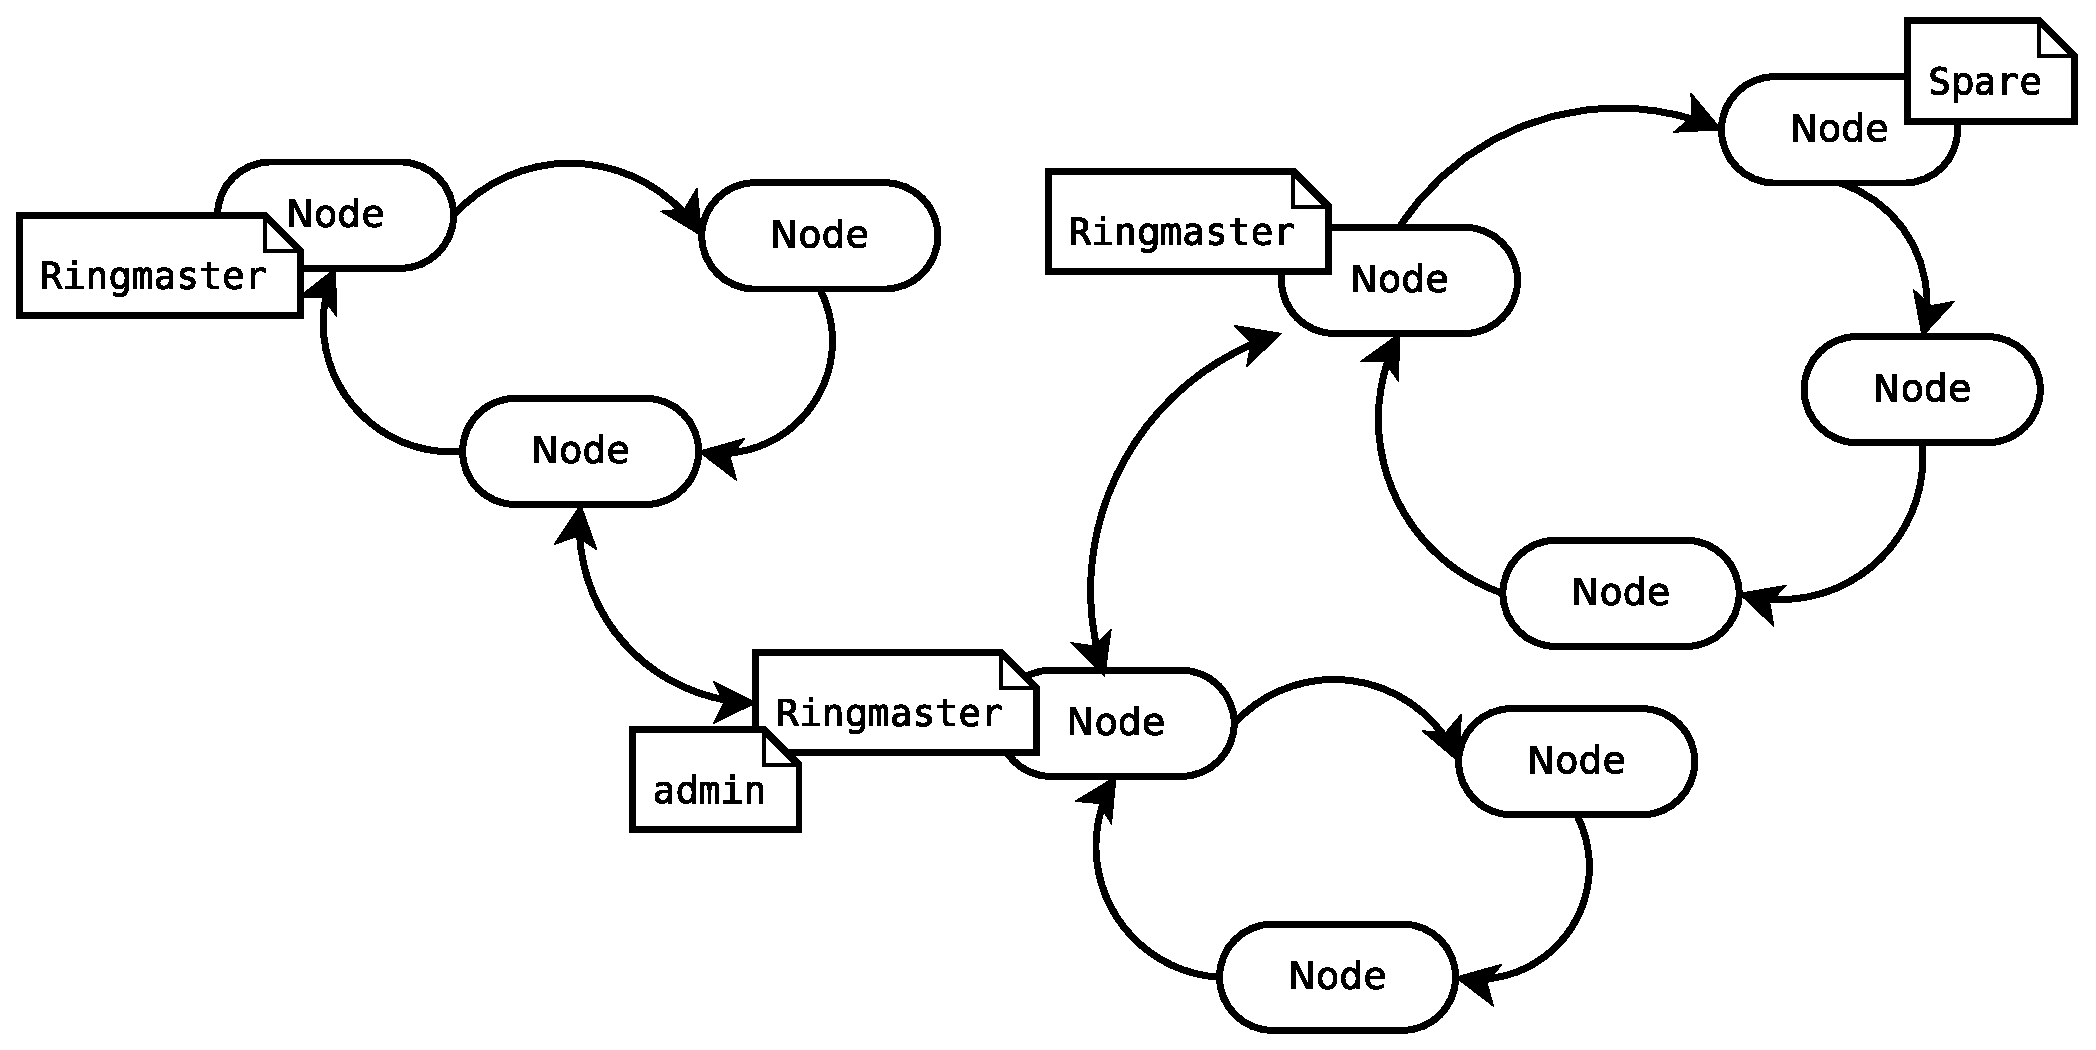
\includegraphics[scale=0.3]{fig/old_topology.eps}
 \caption{Alternate network model}
 \label{fig:old_network_model}
\end{figure}


\end{document}
%TODO References.
%@article{lamport1982byzantine,
%  title={The Byzantine generals problem},
%  author={Lamport, Leslie and Shostak, Robert and Pease, Marshall},
% journal={ACM Transactions on Programming Languages and Systems (TOPLAS)},
%  volume={4},
%  number={3},
%  pages={382--401},
%  year={1982},
%  publisher={ACM}
%}